\section{AngioTK pipeline overview}
\subsection{Goal}

%---------------------------------------------------------------------------------------------------

\begin{frame}{Goal}
 \begin{center}
 \begin{figure}[H]
	\begin{minipage}[b]{0.49\linewidth}
            	\centering
            	\includegraphics[width=\linewidth]{\imgpath 0_mri}
		\caption*{MRA}
	\end{minipage}
	\hfill
	\begin{minipage}[b]{0.49\linewidth}
            	\centering
            	\includegraphics[width=\linewidth]{\imgpath 7_vm}
		\caption*{3D mesh}
	\end{minipage}
 \end{figure}
 	\vfill
	Goal: MRA $\rightarrow$ Blood vessels 3D mesh.
 \end{center}
\end{frame}

%---------------------------------------------------------------------------------------------------

\newcommand{\imgWidth}{.48\linewidth}

\begin{frame}{Intermediary steps}
 \begin{center}
 \begin{figure}[H]
 	\hfill
	\begin{minipage}[b]{\imgWidth}
            	\centering
            	\includegraphics[width=\linewidth]{\imgpath 0_mri}
		\caption*{MRA}
	\end{minipage}
	\begin{minipage}[b]{\imgWidth}
            	\centering
            	\includegraphics[width=\linewidth]{\imgpath 1_rorpo}
		\caption*{Filtering}
	\end{minipage}
	\hfill \hfill
	
	\hfill
	\begin{minipage}[b]{\imgWidth}
            	\centering
            	\includegraphics[width=\linewidth]{\imgpath 2_sfi}
		\caption*{Surface Extraction}
	\end{minipage}
	\begin{minipage}[b]{\imgWidth}
            	\centering
            	\includegraphics[width=\linewidth]{\imgpath 7_vm}
		\caption*{Volume meshing}
	\end{minipage}
	\hfill \hfill
 \end{figure}
 \end{center}
\end{frame}

%---------------------------------------------------------------------------------------------------
\subsection{Problem}
%---------------------------------------------------------------------------------------------------

\renewcommand{\imgWidth}{1\linewidth}

\begin{frame}{Problem}
 \begin{center}
 \begin{figure}[H]
	\begin{minipage}[b]{\imgWidth}
            	\centering
            	\includegraphics[width=\linewidth]{\imgpath 2_sfi}
		\caption*{Extracted surface: noisy...}
	\end{minipage}
 \end{figure}
 \end{center}
\end{frame}

%---------------------------------------------------------------------------------------------------

\renewcommand{\imgWidth}{1\linewidth}

\begin{frame}{Problem}
 \begin{center}
 \begin{figure}[H]
	\begin{minipage}[b]{\imgWidth}
            	\centering
            	\includegraphics[width=\linewidth]{\imgpath 2_sfi_cu}
		\caption*{...and irregular}
	\end{minipage}
 \end{figure}
 \end{center}
\end{frame}

%---------------------------------------------------------------------------------------------------
\subsection{Our solution}
%---------------------------------------------------------------------------------------------------

\begin{frame}{Additional steps: generate a smooth surface using blood vessels center lines}
 Pipeline steps:
 \begin{center}
 \begin{itemize}
 	\item 1 - Filtering
 	\item 2 - Surface extraction
 	\item 3a - Center lines creation 
 	\item 3b - Center lines computing and merging
 	\item 4 - Image generation from center lines 
 	\item 5 - Second surface extraction
 	\item 6 - Surface remeshing
 	\item 7 - Volume meshing
 \end{itemize}
 \end{center}
\end{frame}

%---------------------------------------------------------------------------------------------------

\begin{frame}{Center lines creation tool}
 \begin{center}
 \begin{figure}[H]
 	\begin{minipage}[b]{0.49\linewidth}
            	\centering
            	\includegraphics[width=\linewidth]{\imgpath gui2}
	\end{minipage}
	\hfill
	\begin{minipage}[b]{0.49\linewidth}
            	\centering
            	\includegraphics[width=\linewidth]{\imgpath gui1}
	\end{minipage}
	\caption*{\centering Using this graphical tool, we manually place points throughout the blood vessels...}
 \end{figure}
 \end{center}
\end{frame}

%---------------------------------------------------------------------------------------------------

\begin{frame}{Center lines computing}
 \begin{center}
	\begin{figure}[H]
	\includegraphics[width=.9\linewidth]{\imgpath 3_cl_w}
	\caption*{}
 \end{figure}
 \vfill
 ...and the software generates and merges together the corresponding center lines
 \end{center}
\end{frame}

%---------------------------------------------------------------------------------------------------

\begin{frame}{Image generation using center lines}
 \begin{center}
	\begin{figure}[H]
	\includegraphics[width=\linewidth]{\imgpath 4_ifcl}
	\caption*{We generate a new, noise-free 3D image using the center lines.}
 \end{figure}
 \vfill
 \end{center}
\end{frame}

%---------------------------------------------------------------------------------------------------

\begin{frame}{Image generation using center lines}
 \begin{center}
 \begin{figure}[H]
 	\begin{minipage}[b]{0.49\linewidth}
            	\centering
            	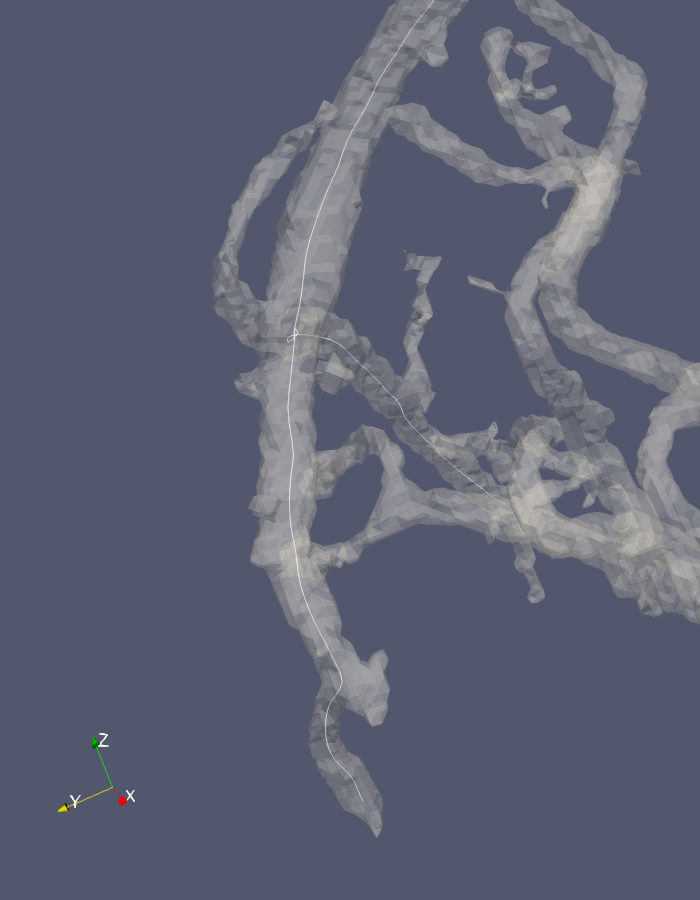
\includegraphics[width=\linewidth]{\imgpath details/3_cl_detail1}
		\caption*{}
	\end{minipage}
	\hfill
	\begin{minipage}[b]{0.49\linewidth}
            	\centering
            	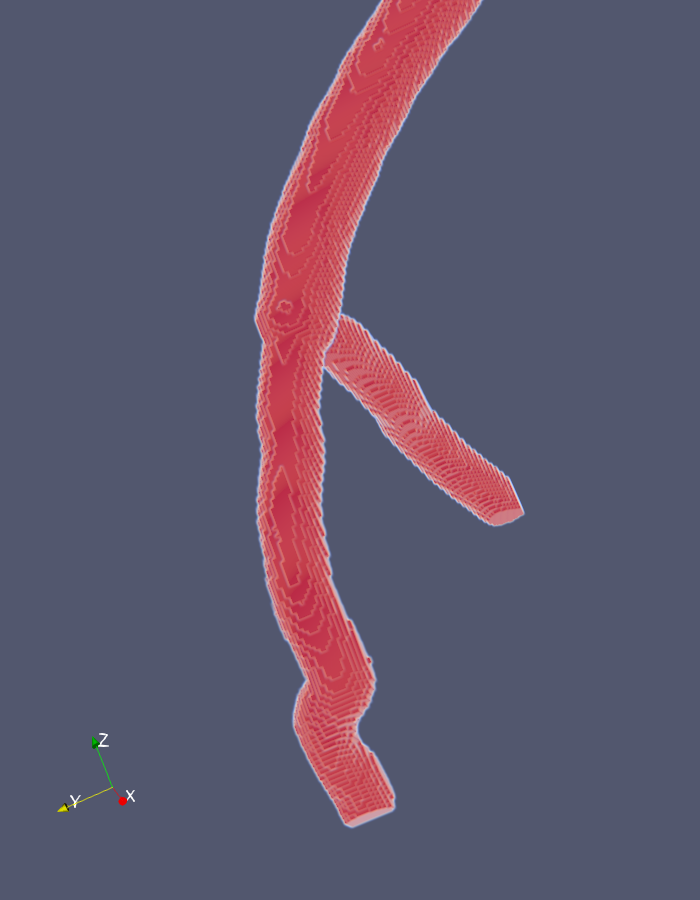
\includegraphics[width=\linewidth]{\imgpath details/4_ifcl_detail1}
		\caption*{}
	\end{minipage}
 \end{figure}
 \end{center}
\end{frame}

%---------------------------------------------------------------------------------------------------

\begin{frame}{Second surface extraction}
 \begin{center}
	\begin{figure}[H]
	\includegraphics[width=.9\linewidth]{\imgpath 5_sfi2}
	\caption*{We can then perform a second surface extraction.}
 \end{figure}
 \end{center}
\end{frame}

%---------------------------------------------------------------------------------------------------

\begin{frame}{Second surface extraction}
 \begin{center}
 \begin{figure}[H]
 	\begin{minipage}[b]{0.45\linewidth}
            	\centering
            	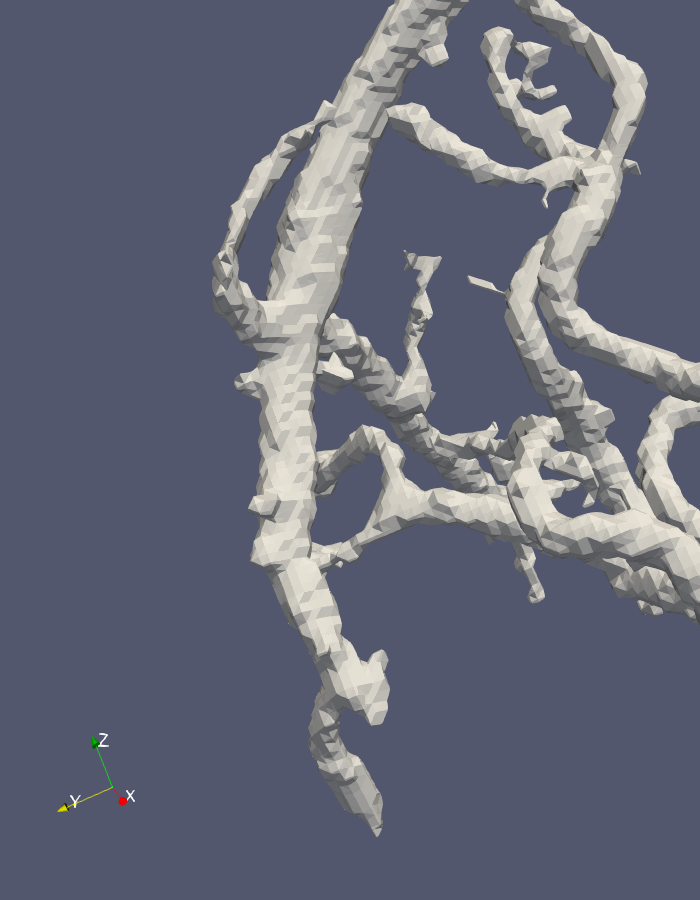
\includegraphics[width=\linewidth]{\imgpath details/2_surface}
	\end{minipage}
	\begin{minipage}[b]{0.45\linewidth}
            	\centering
            	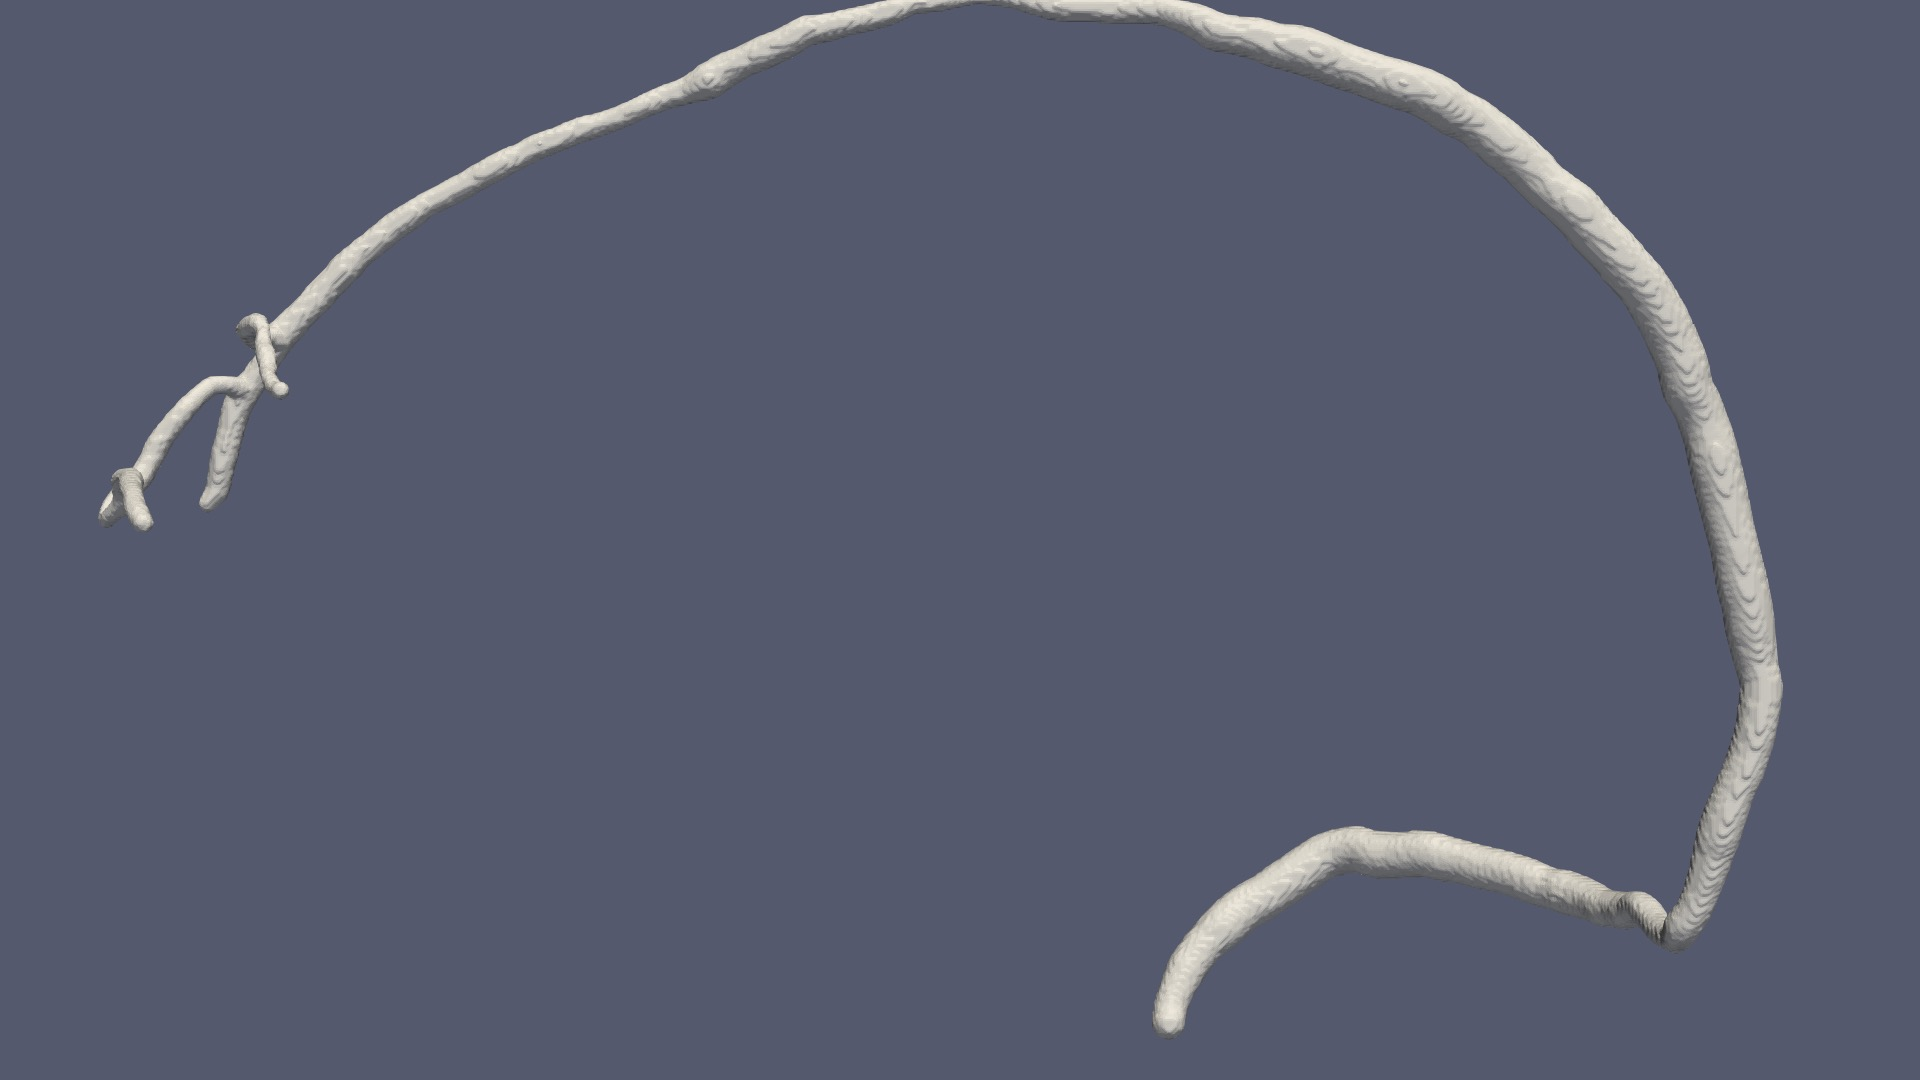
\includegraphics[width=\linewidth]{\imgpath details/5_sfi2}
	\end{minipage}
  	\caption*{This extracted surface is both smoother than the first one and noise-free. }
 \end{figure}
 \end{center}
\end{frame}

%---------------------------------------------------------------------------------------------------

\begin{frame}{Surface remeshing}
 \begin{center}
 \begin{figure}[H]
 	\begin{minipage}[b]{0.45\linewidth}
            	\centering
            	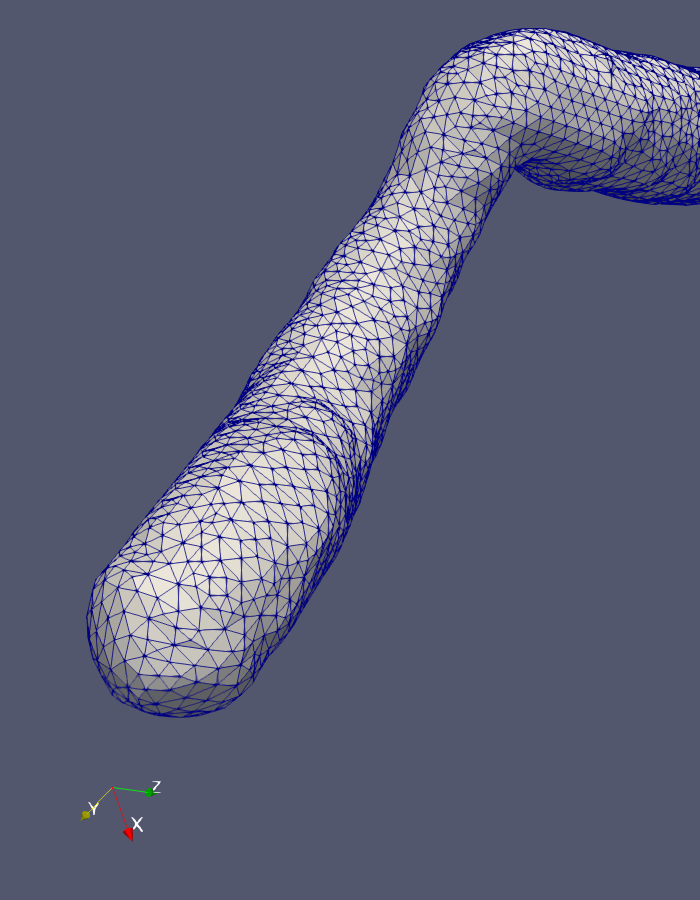
\includegraphics[width=\linewidth]{\imgpath details/5c_sfi2}
	\end{minipage}
	\begin{minipage}[b]{0.45\linewidth}
            	\centering
            	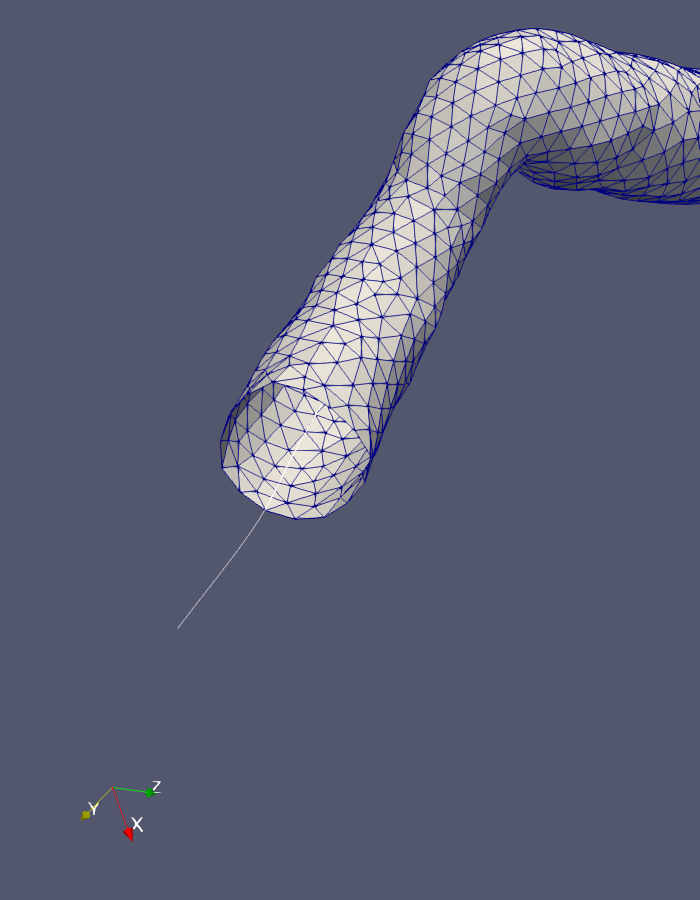
\includegraphics[width=\linewidth]{\imgpath details/6b_sp}
	\end{minipage}
	\caption*{Now, we cut-off the blood vessels ends and remesh the surface.}
 \end{figure}
 \end{center}
\end{frame}

%---------------------------------------------------------------------------------------------------

\begin{frame}{Volume meshing}
 \begin{center}
 \begin{figure}[H]
 	\begin{minipage}[b]{0.45\linewidth}
            	\centering
            	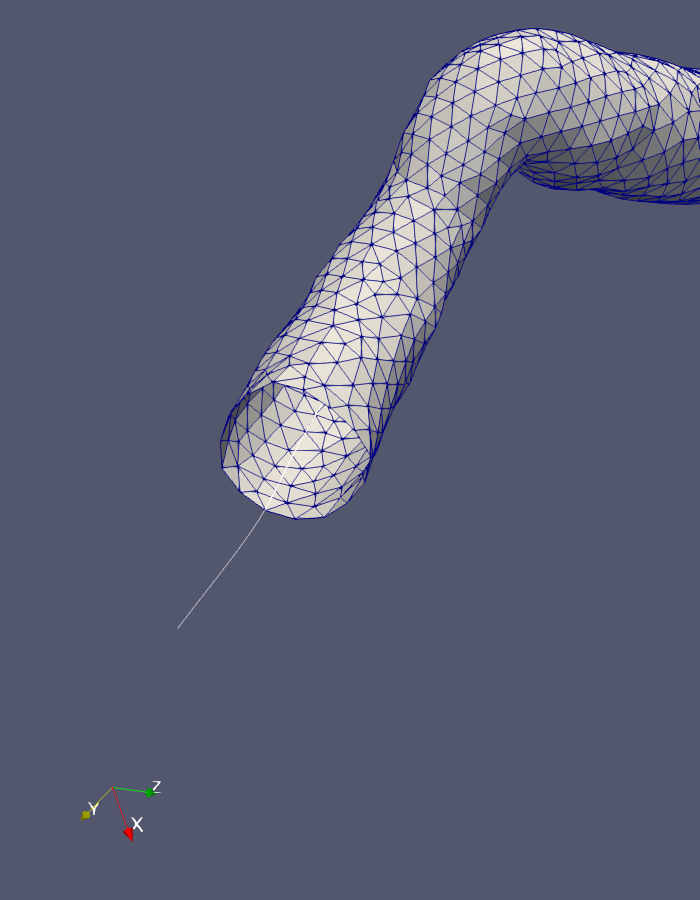
\includegraphics[width=\linewidth]{\imgpath details/6b_sp}
	\end{minipage}
	\begin{minipage}[b]{0.45\linewidth}
            	\centering
            	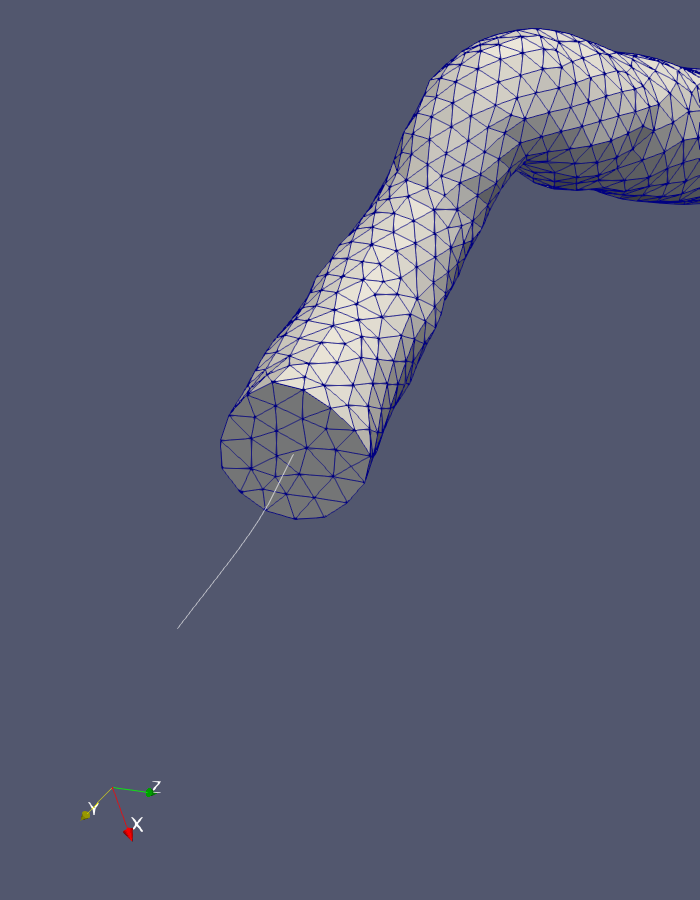
\includegraphics[width=\linewidth]{\imgpath details/7_vp}
	\end{minipage}
	\caption*{The last step is to mesh the volume.}
 \end{figure}
 \end{center}
\end{frame}

%---------------------------------------------------------------------------------------------------

\newcommand{\figpart}{.35}
\newcommand{\hpart}{.35}

\begin{frame}{Comparison}
\begin{center}
 \begin{figure}[H]
	\begin{minipage}[t]{\figpart \linewidth}
            	\centering
            	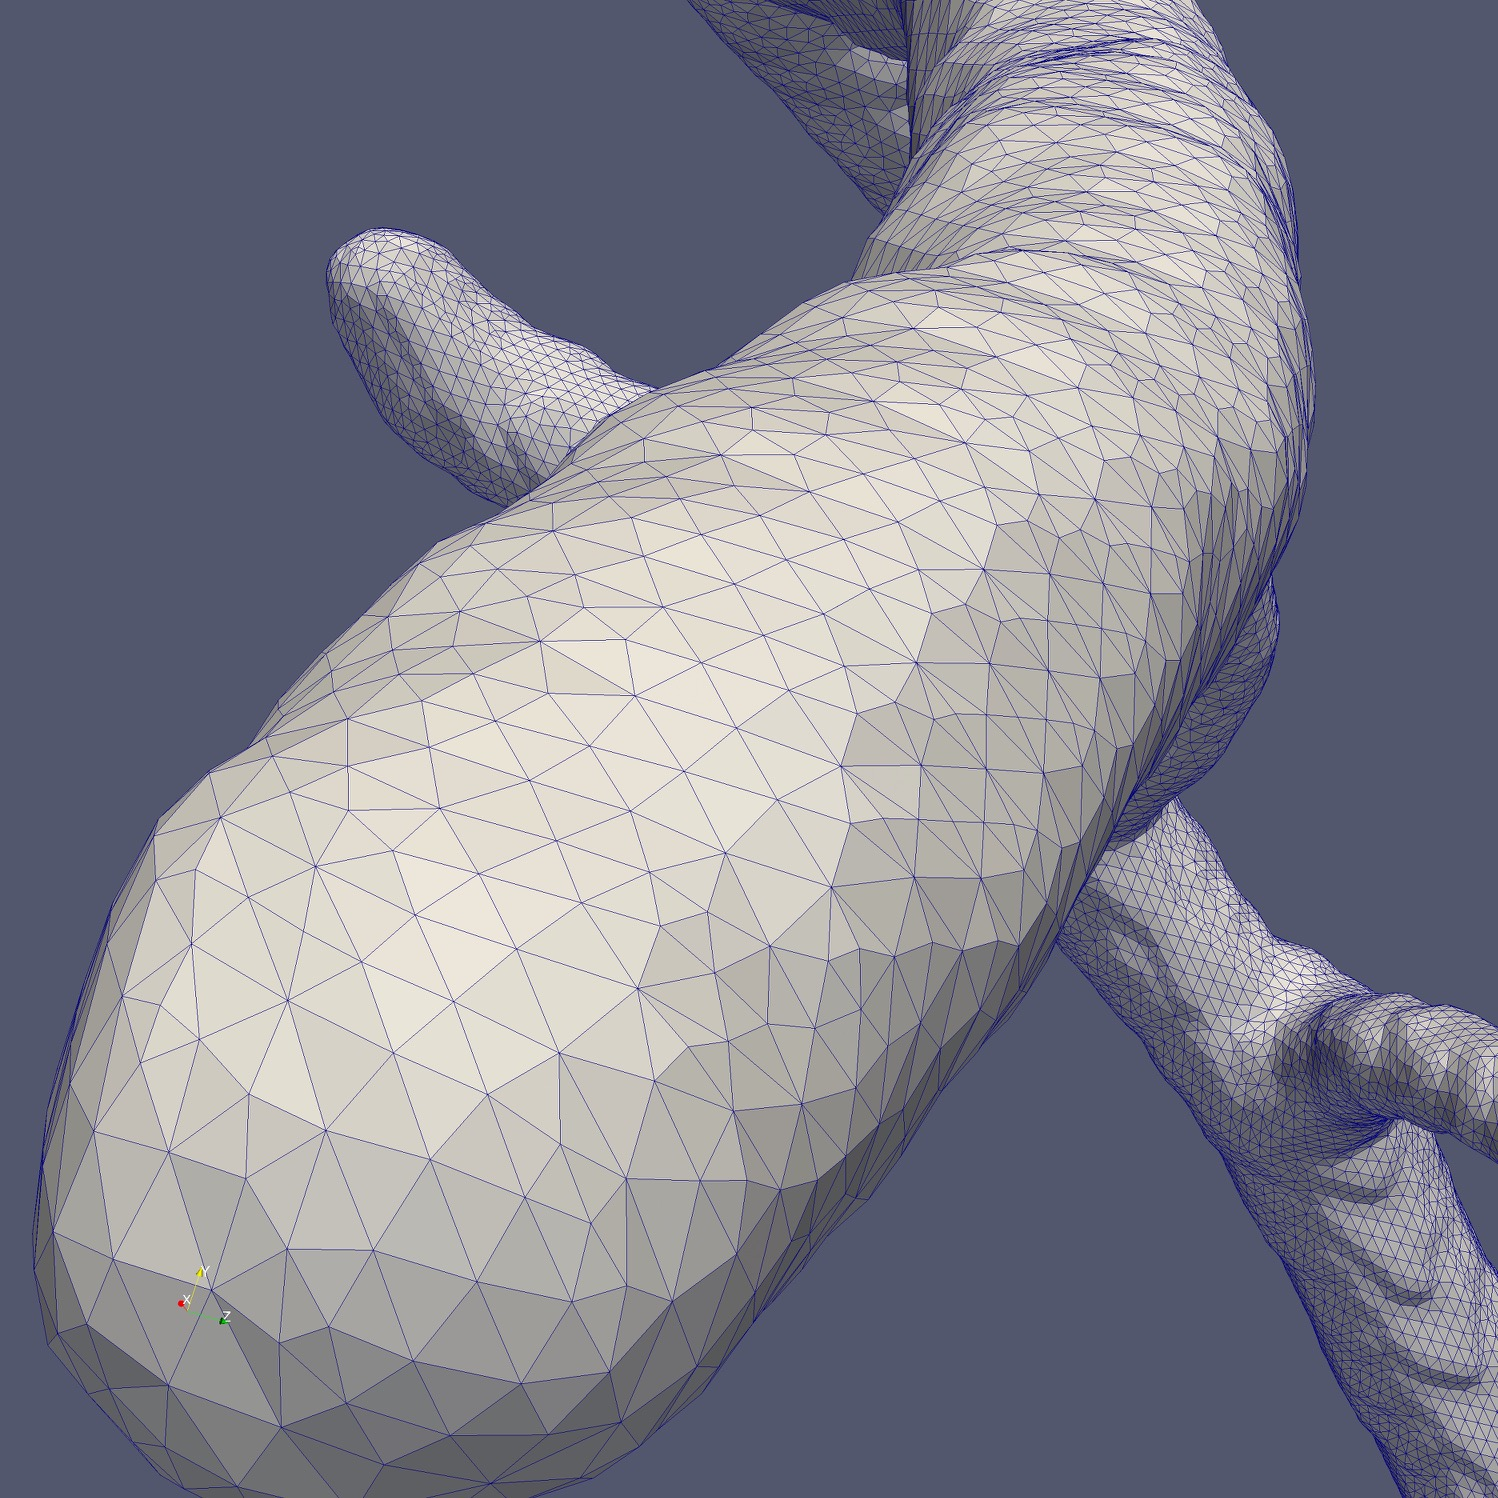
\includegraphics[width=\linewidth,height=\hpart \textheight,keepaspectratio]{\imgpath details/5_sfi2_wf_cu2}
		\caption*{Extracted surface}
	\end{minipage}
	\begin{minipage}[t]{\figpart \linewidth}
            	\centering
            	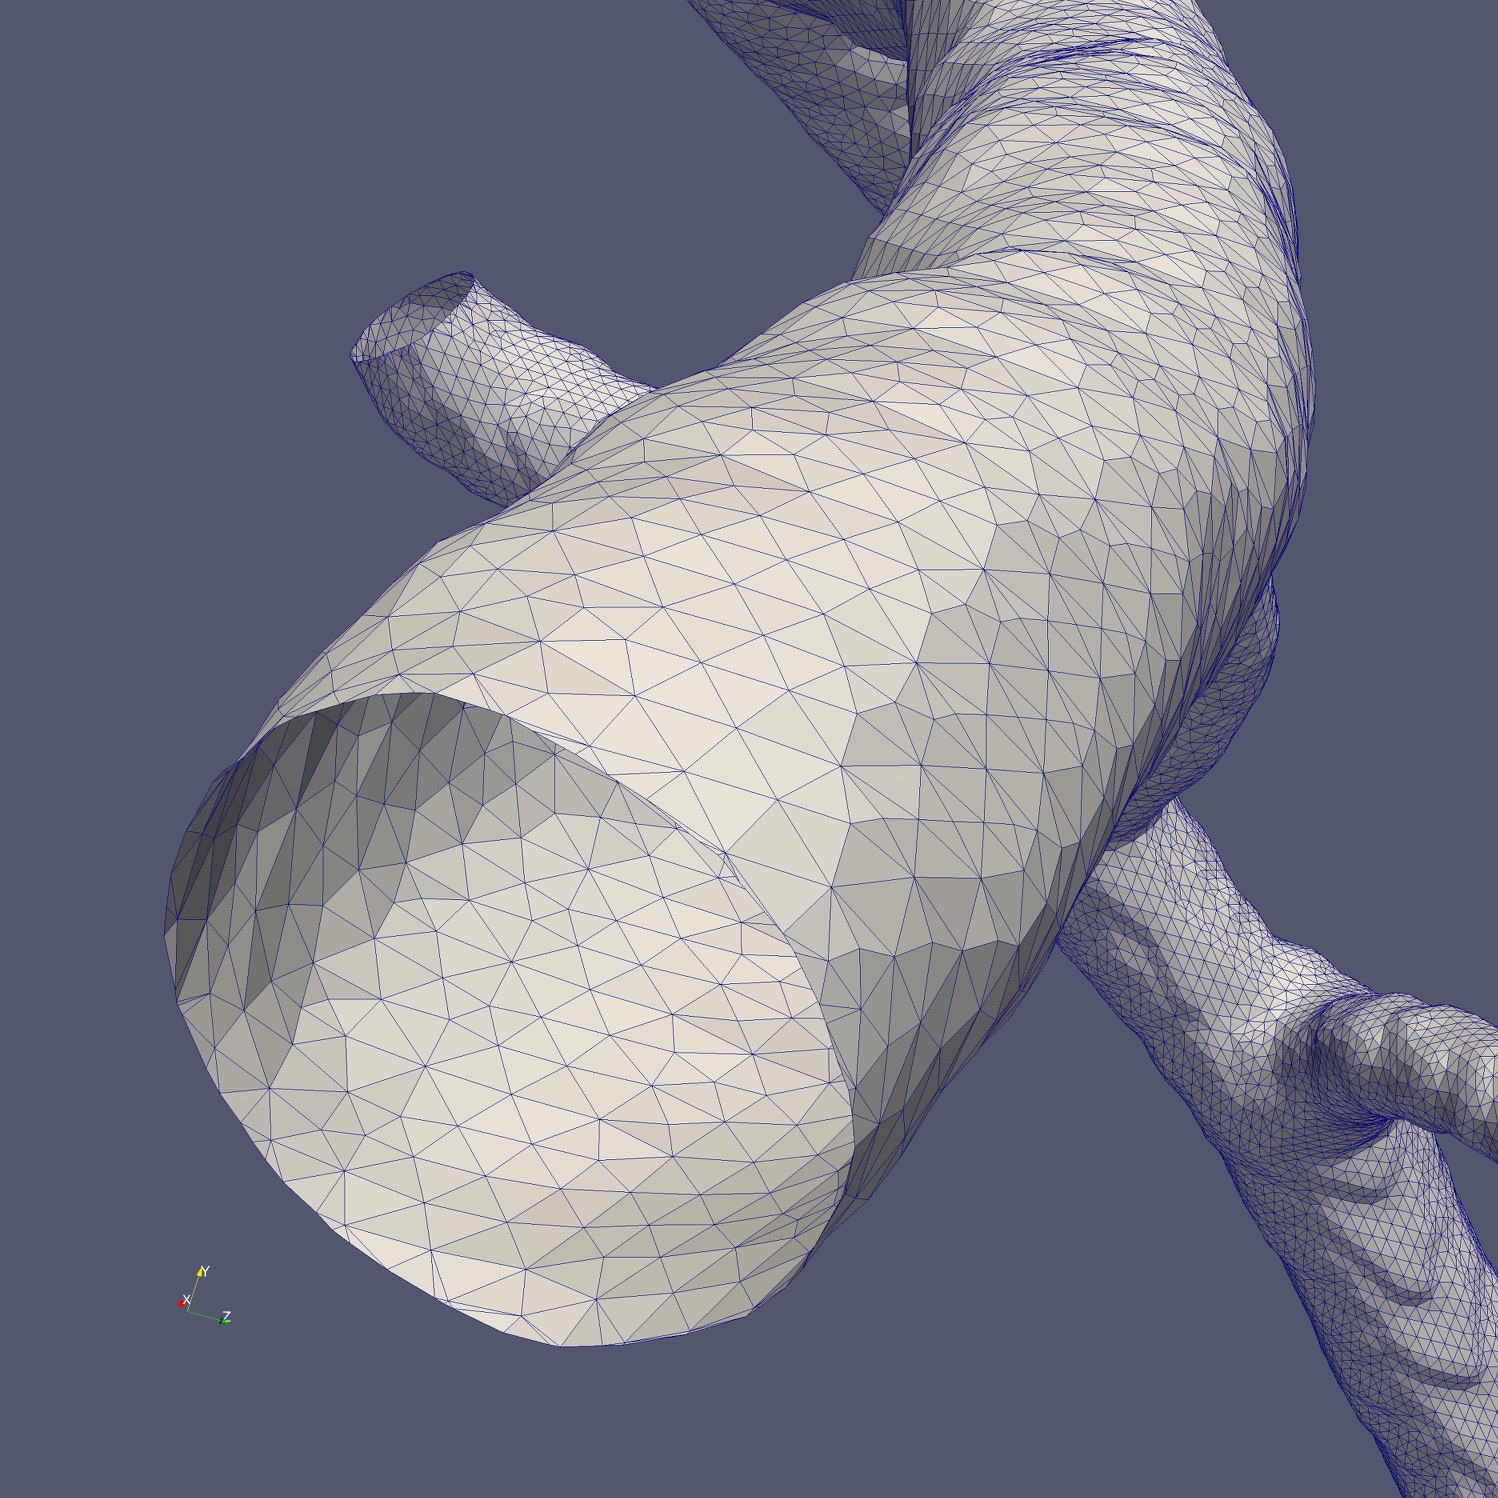
\includegraphics[width=\linewidth,height=\hpart \textheight,keepaspectratio]{\imgpath details/6_sm_open_wf_cu2}
		\caption*{Ends opening}
	\end{minipage}
	\begin{minipage}[t]{\figpart \linewidth}
            	\centering
            	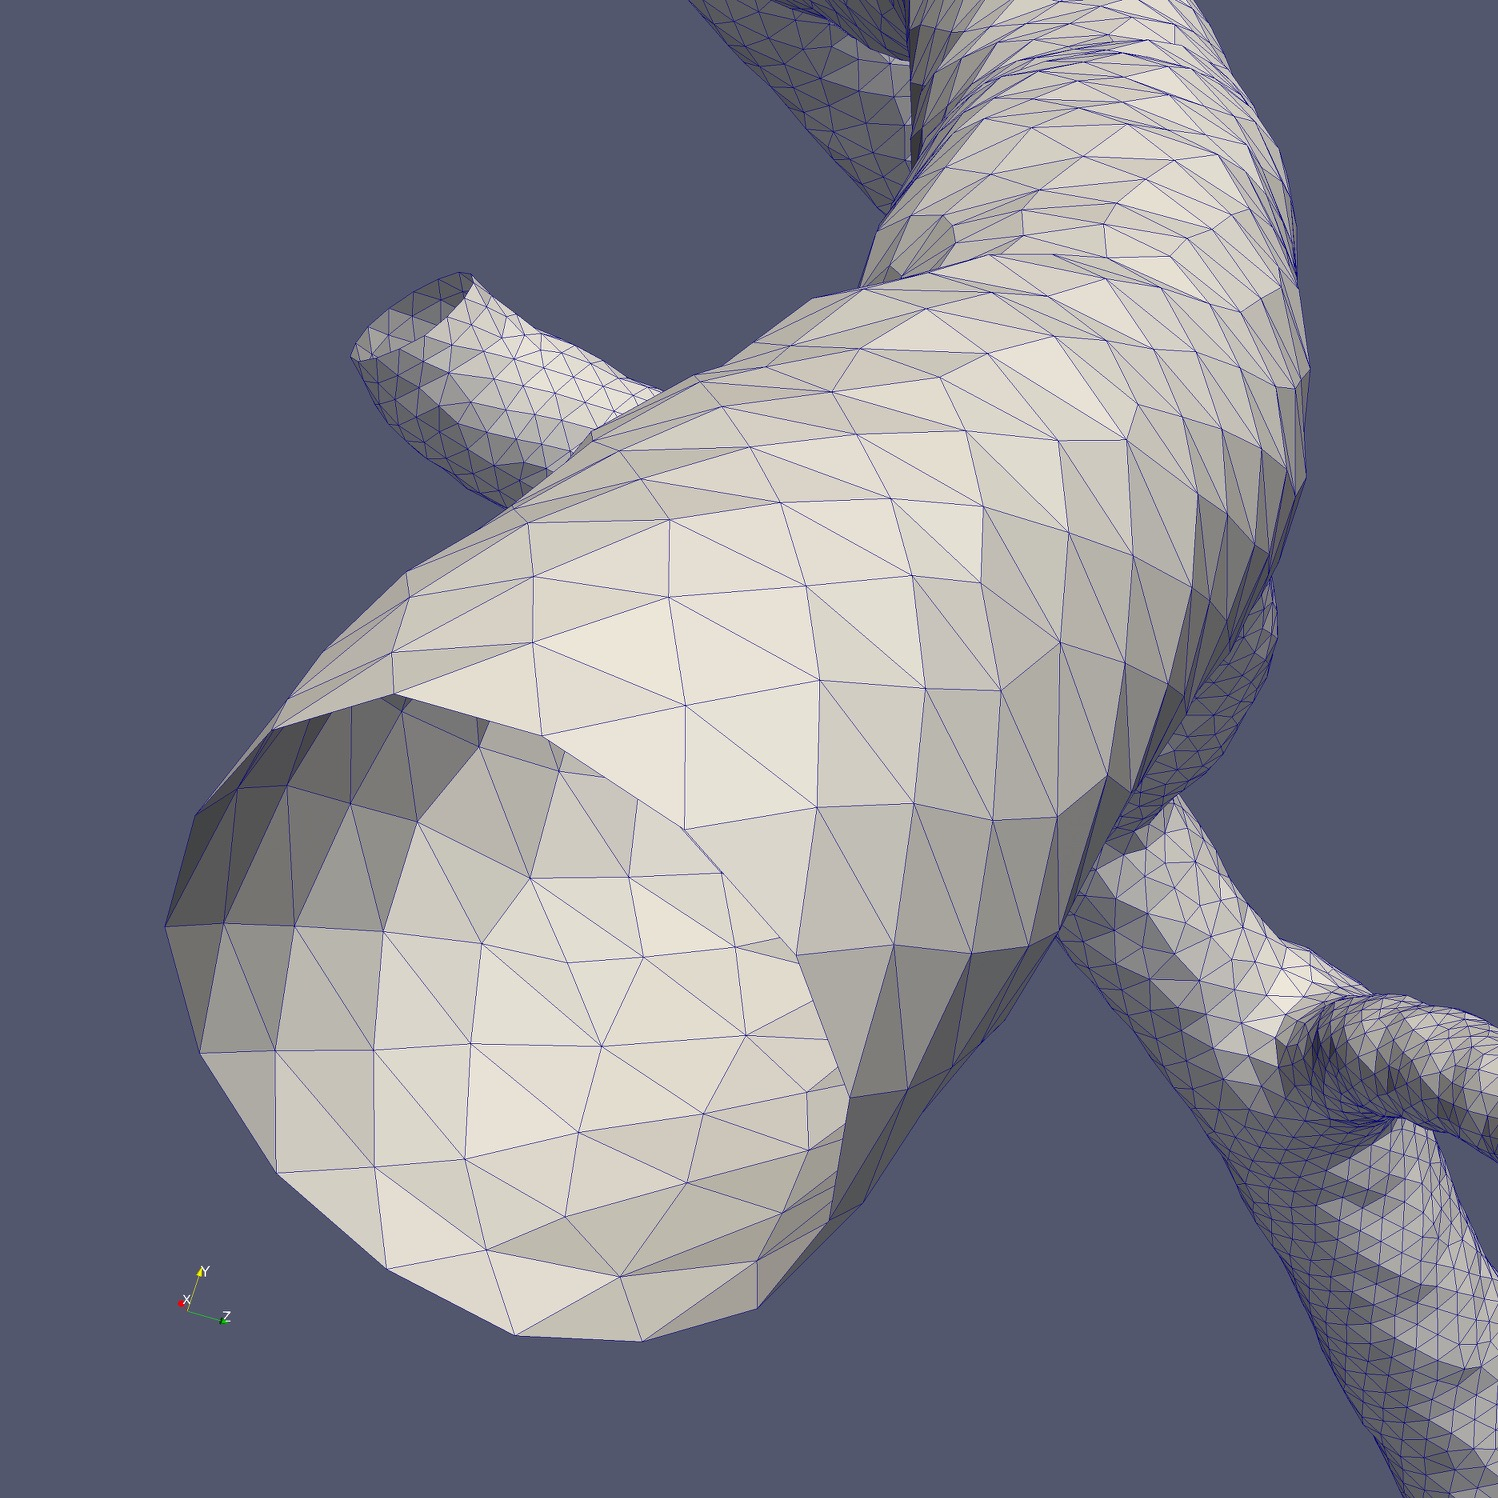
\includegraphics[width=\linewidth,height=\hpart \textheight,keepaspectratio]{\imgpath details/6_sm_remesh_wf_cu2}
		\caption*{Surface remeshing}
	\end{minipage}
	\begin{minipage}[t]{\figpart \linewidth}
            	\centering
            	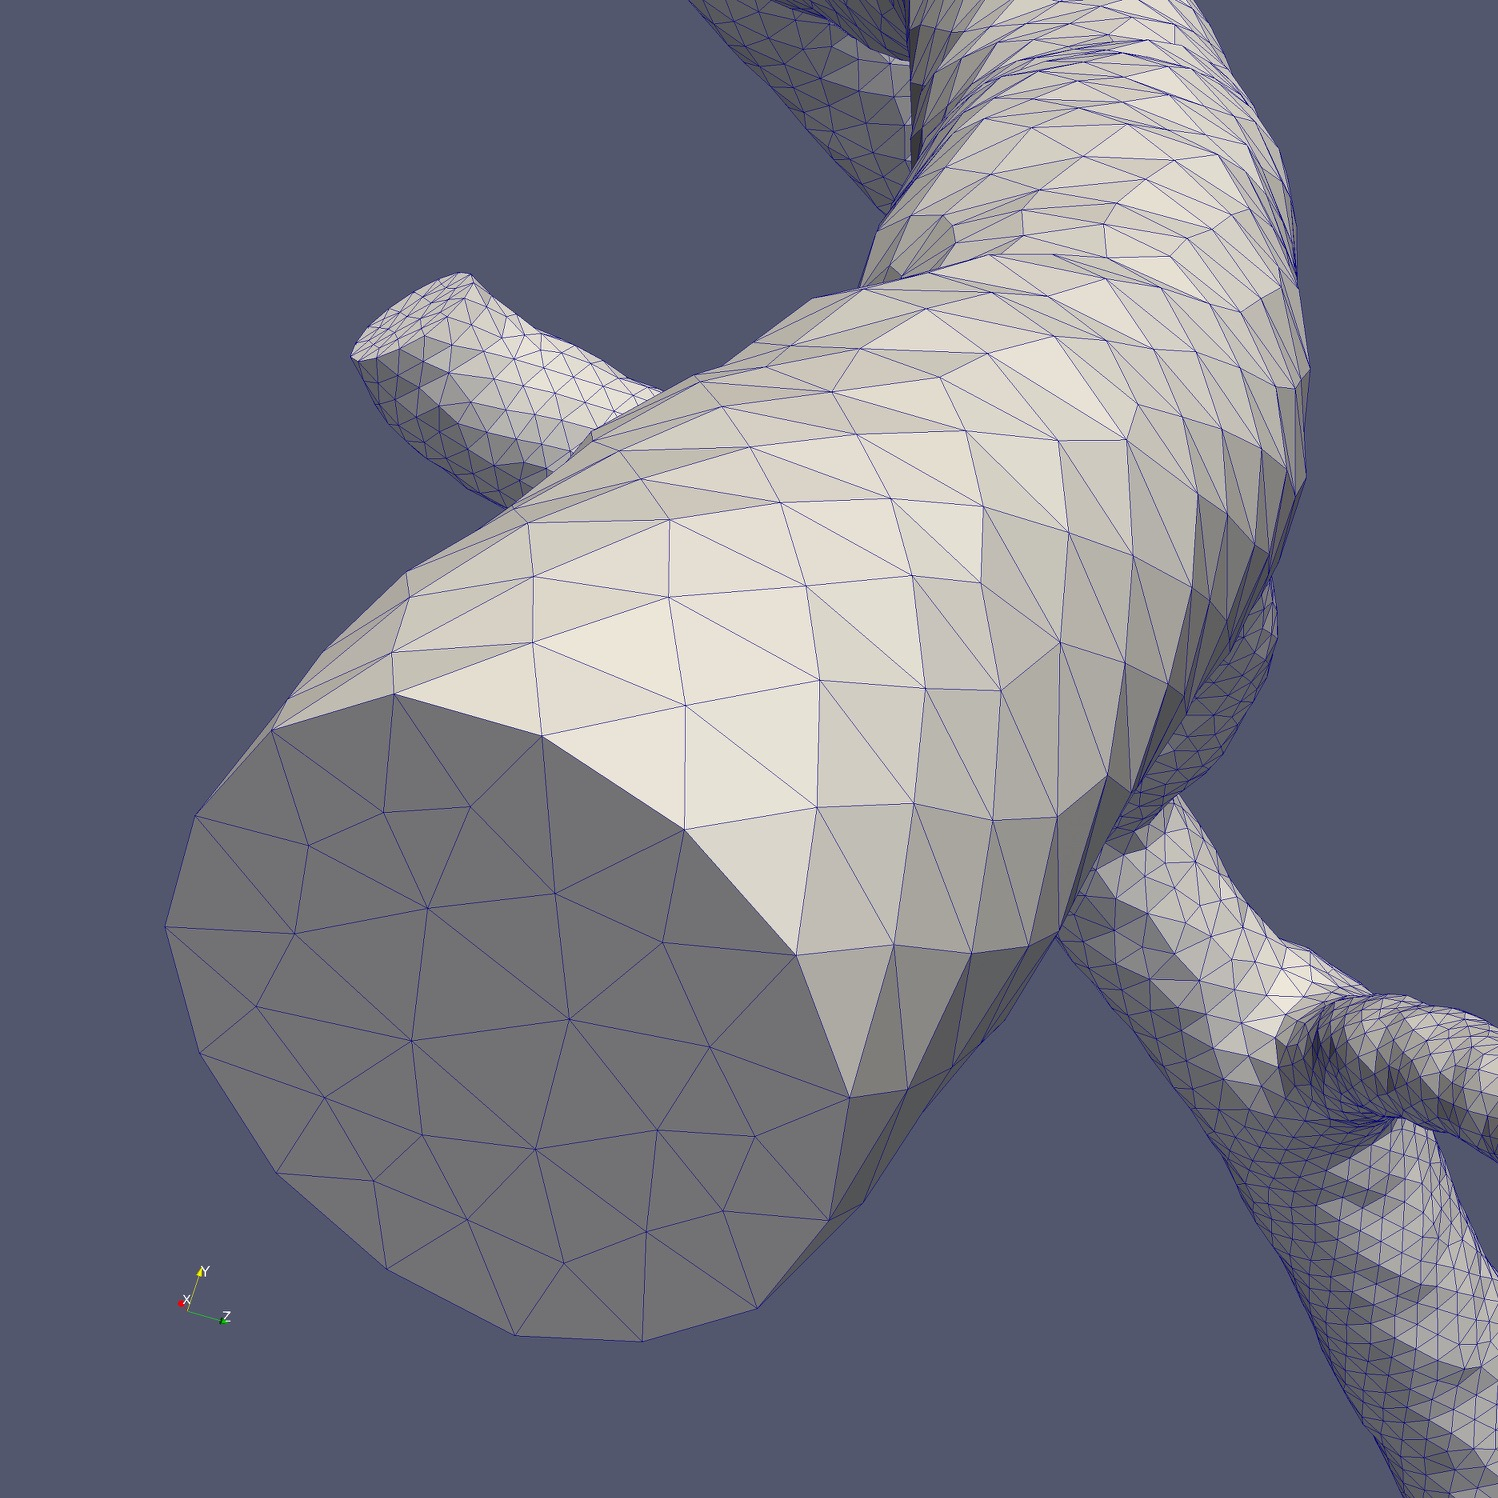
\includegraphics[width=\linewidth,height=\hpart \textheight,keepaspectratio]{\imgpath details/7_vm_wf_cu2}
		\caption*{Volume meshing}
	\end{minipage}
 \end{figure}
\end{center}
\end{frame}

